\chapter{Software Design, State Of The Art} \label{chapter3}
\minitoc
\eject

\cit{A designer is responsible for producing the greatest benefit for any given investment of time, talent, money, and other resources.}{K. Sullivan, W. Griswold, Y. Cai, B. Hallen \cite{Sullivan2001}}

With the growth of Software as a Service (SaaS) on the web, the same company carries both development and exploitation of an application at scale of unprecedented size.
It revealed the importance of previously unknown economic constraints.
To assure the continuous growth and sustainability of an application, it needs to address two contradictory goals : development productivity and performance efficiency.
These goals needs to be enforced by the platform supporting the application to build good development habits for the developers.
% In this chapter,
A platform designates any solution that allows to build an application on top of it, including programming languages, compilers, interpreters, frameworks, runtime libraries and so on.

\textit{75\% of your budget is dedicated to software maintenance.}\ftnt{http://www.castsoftware.com/glossary/software-maintainability}
The productivity of a platform is the degree to which developers can quickly produce new and modify existing software.
It impacts the maintainability of the applications and relies on the modularity enforced by its platform.
Especially, higher order programming is crucial to build and compose modules productively.
It relies either on mutable states, or immutable states, but hardly on a combination of both.

However, neither mutable nor immutable states allows performance efficiency.
Mutable states leads to synchronization overhead at a coarser-grain level, while immutable states leads to communication overhead at a finer-grain level.
Efficiency relies on a combination of synchronization at a fine-grain level, and immutable message passing at a coarse-grain level.
This combination breaks the modularity, hence the productivity of an application.
A company has no choice but to commit huge development efforts to get efficient performances.

\illustration{virtuous circle between community and industry}
Moreover, a balance between productivity and efficiency is required for a platform to enter a virtuous circle of adoption.
The productivity is required to be appealing to gather a community to support the ecosystem around the platform.
This community is appealing for the industry as a hiring pool.
Additionally, the efficiency is required to be adopted by the industry to be economically viable.
And the industrial relevance provides the reason for this ecosystem to exist and the community to gather.

This chapter presents a broad view of the state of the art in the compromises between productivity and efficiency.
It defines software productivity, efficiency, and adoption in section \ref{chapter3:definitions} and all the underlying concepts, such as higher order programming and state mutability.
It then analyzes different platforms according to their focus. platforms focusing on productivity are addressed in section \ref{chapter3:software-productivity}, those focusing on efficiency in section \ref{chapter3:software-efficiency} and those focusing on a compromise between the two in section \ref{chapter3:software-abstraction}.

\DTLsetseparator{ | }
\DTLloaddb{platforms}{../../data/platforms-analysis.csv}

\newcommand{\ExtractGroup}[2]{% Name of the group, Headers
\DTLforeach*[ %
    \equal{\Group}{#1} %
  ]{platforms}{ %
    \Group=Group, %
    \Model=Model, %
    \Implementations=Implementations, %
    \Composition=Composition, %
    \Encapsulation=Encapsulation, %
    \Maintainability=Maintainability, %
    \Synchronization=Synchronization, %
    \Message=Message, %
    \Performance=Performance, %
    \Community=Community, %
    \Industry=Industry, %
    \Adoption=Adoption}
  {\DTLiffirstrow{}{\\\tabucline[on .5pt]{-}}#2}
  \\\tabucline[.5pt]{-}
}

%% -------------------------------------------------------------------------------------------
%%                                          SCHEMAS
%% -------------------------------------------------------------------------------------------

% MAINTAINABILITY
\newcommand{\MaintainabilityCol}    {4}
\newcommand{\MaintainabilityHeader} { Model &  Implementations &   \lab{Composition} &   \lab{Encapsulation} & $\to$ &   \lab{Maintainability} \\ \tabucline[.5pt]{-} }
\newcommand{\MaintainabilityRow}    {\Model & \Implementations & \rate{\Composition} & \rate{\Encapsulation} &&        \rate{\Maintainability}}

% PERFORMANCE
\newcommand{\PerformanceCol}        {4}
\newcommand{\PerformanceHeader}     { Model &  Implementations & \lab{Fine-grain level synchronization} & \lab{Coarse-grain level message passing} & $\to$ & \lab{Performance Efficiency} \\ \tabucline[.5pt]{-} }
\newcommand{\PerformanceRow}        {\Model & \Implementations & \rate{\Synchronization}                & \rate{\Message}                          &&      \rate{\Performance}}

% ADOPTION
\newcommand{\AdoptionCol}           {4}
\newcommand{\AdoptionHeader}        { Model &  Implementations &   \lab{Community support} &   \lab{Industrial need} & $\to$ &   \lab{Adoption} \\ \tabucline[.5pt]{-} }
\newcommand{\AdoptionRow}           {\Model & \Implementations & \rate{\Community}         & \rate{\Industry}        &&        \rate{\Adoption}}

% SUMMARY
\newcommand{\SummaryCol}            {3}
\newcommand{\SummaryHeader}         { Model &  Implementations  &   \lab{Maintainability} &   \lab{Adoption} &   \lab{Performance Efficiency} \\ \tabucline[.5pt]{-} }
\newcommand{\SummaryRow}            {\Model & \Implementations  & \rate{\Maintainability} & \rate{\Adoption} & \rate{\Performance}}

%% -------------------------------------------------------------------------------------------
%%                                       EXTRACTIONS
%% -------------------------------------------------------------------------------------------

% MAINTAINABILITY
\newcommand{\ModularMaintainability}    {\ExtractGroup{Modular}    {\MaintainabilityRow}}
\newcommand{\ConcurrentMaintainability} {\ExtractGroup{Concurrent} {\MaintainabilityRow}}
\newcommand{\ParallelMaintainability}   {\ExtractGroup{Parallel}   {\MaintainabilityRow}}
\newcommand{\StreamMaintainability}     {\ExtractGroup{Stream}     {\MaintainabilityRow}}
\newcommand{\RuntimeMaintainability}    {\ExtractGroup{Runtime}    {\MaintainabilityRow}}
\newcommand{\CompilerMaintainability}   {\ExtractGroup{Compiler}   {\MaintainabilityRow}}
% PERFORMANCE
\newcommand{\ModularPerformance}        {\ExtractGroup{Modular}    {\PerformanceRow}}
\newcommand{\ConcurrentPerformance}     {\ExtractGroup{Concurrent} {\PerformanceRow}}
\newcommand{\ParallelPerformance}       {\ExtractGroup{Parallel}   {\PerformanceRow}}
\newcommand{\StreamPerformance}         {\ExtractGroup{Stream}     {\PerformanceRow}}
\newcommand{\RuntimePerformance}        {\ExtractGroup{Runtime}    {\PerformanceRow}}
\newcommand{\CompilerPerformance}       {\ExtractGroup{Compiler}   {\PerformanceRow}}
% ADOPTION
\newcommand{\ModularAdoption}           {\ExtractGroup{Modular}    {\AdoptionRow}}
\newcommand{\ConcurrentAdoption}        {\ExtractGroup{Concurrent} {\AdoptionRow}}
\newcommand{\ParallelAdoption}          {\ExtractGroup{Parallel}   {\AdoptionRow}}
\newcommand{\StreamAdoption}            {\ExtractGroup{Stream}     {\AdoptionRow}}
\newcommand{\RuntimeAdoption}           {\ExtractGroup{Runtime}    {\AdoptionRow}}
\newcommand{\CompilerAdoption}          {\ExtractGroup{Compiler}   {\AdoptionRow}}
% SUMMARY
\newcommand{\ModularSummary}            {\ExtractGroup{Modular}    {\SummaryRow}}
\newcommand{\ConcurrentSummary}         {\ExtractGroup{Concurrent} {\SummaryRow}}
\newcommand{\ParallelSummary}           {\ExtractGroup{Parallel}   {\SummaryRow}}
\newcommand{\StreamSummary}             {\ExtractGroup{Stream}     {\SummaryRow}}
\newcommand{\RuntimeSummary}            {\ExtractGroup{Runtime}    {\SummaryRow}}
\newcommand{\CompilerSummary}           {\ExtractGroup{Compiler}   {\SummaryRow}}

%% -------------------------------------------------------------------------------------------
%%                                       TABLES
%% -------------------------------------------------------------------------------------------

%% MODULAR

\newcommand{\ModularMaintainabilityTable}[1]{
  \begin{table}[H]
  \tikzexternaldisable
  \begin{tabu} to \linewidth {@{} l X[l] *{\the\numexpr\MaintainabilityCol}{c} @{}}
  \MaintainabilityHeader
  \ModularMaintainability
  \end{tabu}
  \tikzexternalenable
  \caption{Maintainability of Modular Programming Platforms}
  \label{#1}
  \end{table}
}

\newcommand{\ModularAdoptionTable}[1]{
  \begin{table}[H]
  \tikzexternaldisable
  \begin{tabu} to \linewidth {@{} l X[l] *{\the\numexpr\AdoptionCol}{c} @{}}
  \AdoptionHeader
  \ModularAdoption
  \end{tabu}
  \tikzexternalenable
  \caption{Adoption of Modular Programming Platforms}
  \label{#1}
  \end{table}
}

\newcommand{\ModularPerformanceTable}[1]{
  \begin{table}[H]
  \tikzexternaldisable
  \begin{tabu} to \linewidth {@{} l X[l] *{\the\numexpr\PerformanceCol}{c} @{}}
  \PerformanceHeader
  \ModularPerformance
  \end{tabu}
  \tikzexternalenable
  \caption{Performance Efficiency of Modular Programming Platforms}
  \label{#1}
  \end{table}
}

\newcommand{\ModularSummaryTable}[1]{
  \begin{table}[H]
  \tikzexternaldisable
  \begin{tabu} to \linewidth {@{} l X[l] *{\the\numexpr\SummaryCol}{c} @{}}
  \SummaryHeader
  \ModularSummary
  \end{tabu}
  \tikzexternalenable
  \caption{Summary of Modular Programming Platforms}
  \label{#1}
  \end{table}
}

%% PERFORMANCE

\newcommand{\ConcurrentPerformanceTable}[1]{
  \begin{table}[H]
  \tikzexternaldisable
  \begin{tabu} to \linewidth {@{} l X[l] *{\the\numexpr\PerformanceCol}{c} @{}}
  \PerformanceHeader
  \ConcurrentPerformance
  \end{tabu}
  \tikzexternalenable
  \caption{Performance Efficiency of Concurrent Programming Platforms}
  \label{#1}
  \end{table}
}

\newcommand{\ParallelPerformanceTable}[1]{
  \begin{table}[H]
  \tikzexternaldisable
  \begin{tabu} to \linewidth {@{} l X[l] *{\the\numexpr\PerformanceCol}{c} @{}}
  \PerformanceHeader
  \ConcurrentPerformance
  \ParallelPerformance
  \end{tabu}
  \tikzexternalenable
  \caption{Performance Efficiency of Concurrent and Parallel Programming Platforms}
  \label{#1}
  \end{table}
}

\newcommand{\ConcurrentAdoptionTable}[1]{
  \begin{table}[H]
  \tikzexternaldisable
  \begin{tabu} to \linewidth {@{} l X[l] *{\the\numexpr\AdoptionCol}{c} @{}}
  \AdoptionHeader
  \ConcurrentAdoption
  \end{tabu}
  \tikzexternalenable
  \caption{Adoption of Concurrent Programming Platforms}
  \label{#1}
  \end{table}
}

\newcommand{\ParallelAdoptionTable}[1]{
  \begin{table}[H]
  \tikzexternaldisable
  \begin{tabu} to \linewidth {@{} l X[l] *{\the\numexpr\AdoptionCol}{c} @{}}
  \AdoptionHeader
  \ConcurrentAdoption
  \ParallelAdoption
  \end{tabu}
  \tikzexternalenable
  \caption{Adoption of Concurrent and Parallel Programming Platforms}
  \label{#1}
  \end{table}
}

\newcommand{\PerformanceMaintainabilityTable}[1]{
  \begin{table}[H]
  \tikzexternaldisable
  \begin{tabu} to \linewidth {@{} l X[l] *{\the\numexpr\MaintainabilityCol}{c} @{}}
  \MaintainabilityHeader
  \ConcurrentMaintainability
  \ParallelMaintainability
  \StreamMaintainability
  \end{tabu}
  \tikzexternalenable
  \caption{Maintainability of Concurrent, Parallel and Stream Programming Platforms}
  \label{#1}
  \end{table}
}

\newcommand{\PerformanceSummaryTable}[1]{
  \begin{table}[H]
  \tikzexternaldisable
  \begin{tabu} to \linewidth {@{} l X[l] *{\the\numexpr\SummaryCol}{c} @{}}
  \SummaryHeader
  \ConcurrentSummary
  \ParallelSummary
  \StreamSummary
  \end{tabu}
  \tikzexternalenable
  \caption{Summary of Concurrent and Parallel Programming Platforms}
  \label{#1}
  \end{table}
}

%% ABSTRACTION

\newcommand{\AbstractionMaintainabilityTable}[1]{
  \begin{table}[H]
  \tikzexternaldisable
  \begin{tabu} to \linewidth {@{} l X[l] *{\the\numexpr\MaintainabilityCol}{c} @{}}
  \MaintainabilityHeader
  \RuntimeMaintainability
  \CompilerMaintainability
  \end{tabu}
  \tikzexternalenable
  \caption{Maintainability of Compilation and Runtime Platforms}
  \label{#1}
  \end{table}
}

\newcommand{\AbstractionAdoptionTable}[1]{
  \begin{table}[H]
  \tikzexternaldisable
  \begin{tabu} to \linewidth {@{} l X[l] *{\the\numexpr\AdoptionCol}{c} @{}}
  \AdoptionHeader
  \RuntimeAdoption
  \CompilerAdoption
  \end{tabu}
  \tikzexternalenable
  \caption{Adoption of Compilation and Runtime Platforms}
  \label{#1}
  \end{table}
}

\newcommand{\AbstractionPerformanceTable}[1]{
  \begin{table}[H]
  \tikzexternaldisable
  \begin{tabu} to \linewidth {@{} l X[l] *{\the\numexpr\PerformanceCol}{c} @{}}
  \PerformanceHeader
  \RuntimePerformance
  \CompilerPerformance
  \end{tabu}
  \tikzexternalenable
  \caption{Performance Efficiency of Compilation and Runtime Platforms}
  \label{#1}
  \end{table}
}

\newcommand{\AbstractionSummaryTable}[1]{
  \begin{table}[H]
  \tikzexternaldisable
  \begin{tabu} to \linewidth {@{} l X[l] *{\the\numexpr\SummaryCol}{c} @{}}
  \SummaryHeader
  \RuntimeSummary
  \CompilerSummary
  \end{tabu}
  \tikzexternalenable
  \caption{Summary of Compilation and Runtime Platforms}
  \label{#1}
  \end{table}
}

%% Summary

\newcommand{\TableSummary}{ \tikzexternaldisable
  \begin{longtabu} to \linewidth {@{} l X[l] *{\the\numexpr\SummaryCol}{c} @{}}
  \SummaryHeader 
  \ModularSummary
  \ConcurrentSummary
  \ParallelSummary
  \StreamSummary
  \RuntimeSummary
  \CompilerSummary
  \caption{Maintainability of Modular Programming Platforms}
  \label{tab:maintainability-modularity}
  \end{longtabu} \tikzexternalenable
}


\section{Definitions} \label{chapter3:definitions}

The continuous growth and sustainability offered by a platform relies on three criteria.
This section defines these tree criteria, as well as all the underlying concepts.

Additionally, for the context of this thesis, a fourth criterium appear.
It is important for the analyzed platforms to be web compliant.\nt{I don't know where to put this criterium}

\begin{itemize}
\item Maintainability
\item Performance Efficiency
\item Adoption
\item Web compliance
\end{itemize}

\subsection{Maintainability}

\textit{Software maintainability is defined as the degree to which an application is understood, repaired, or enhanced.}\ftnt{http://www.castsoftware.com/glossary/software-maintainability}
% For an application to be maintainable, it needs to be modular.
%Maintainability relies on modularity.
For an application to be maintainable, its frameworks need to enforce modularity directly in the design.
Modularity allows to limit the understanding required to contribute to a module \cite{Stevens1974}.
Which helps developers to repair and enhance the application. 
Moreover, it reduces development time by allowing several developers to simultaneously implement different modules \cite{Wong2009,Cataldo2006}.
% It relies on two factors, module encapsulation and module composition.

\subsubsection{Modularity}

The modularity of a software implementation is about encapsulating subproblems and composing them.
It allows greater design to emerge from the composition of smaller components.

The criteria to define modules to improve maintainability are low coupling and high cohesion \cite{Stevens1974}.
Coupling defines the strength of the interdependence between modules.
Cohesion defines how strongly the features inside a module are related.
% Encapsulating a subproblem into a module helps increase cohesion.
% Composition abstractions helps decrease their coupling.
The composition of modules help decrease coupling, and encapsulation helps increase their cohesion.
Encapsulation and composition improves maintainability.

\begin{itemize}
\item Encapsulation $\to$ High Cohesion
\item Composition $\to$ Low Coupling
\end{itemize}

\subsubsection{Encapsulation}

\paragraph{Boundary Definition}

\illustration{spaghetti programming}
Modular Programming stands upon Structured Programming \cite{Dijkstra1970}.
% Dijkstra firstly developed the concept of Structured Programming \cite{Dijkstra1970}, which later led to modular programming.
% It is defined as \textit{the systematic use of abstraction to control a mass of details, and also a means of documentation which aids program design} \cite{Knuth1974}.
It draws clear interfaces around a piece of implementation so that the execution is enclosed inside.
At a fine level, it helps avoid spaghetti code \cite{Dijkstra1968a}, and at a coarser level, it structures the implementation \cite{Dijkstra1968} into modules, or layers.
% The next paragraph explains further the criteria to draw the borders around modules.

\paragraph{Data Protection}

\illustration{lasagna programming}
Encapsulate a specific design choice in each module, so that it is responsible for one and only one concern, isolate its evolution from impacting the rest of the implementation \cite{Parnas1972, Tarr1999, Hursch1995}.
Examples of such separation of concerns are the separation of the form and the content in HTML / CSS, or the OSI model for the network stack.

\subsubsection{Composition} \label{chapter3:software-maintainability:modularity:features}

\paragraph{Higher-Order Programming}
\nt{If possible, include this reference : Continuations and coroutines \cite{Haynes1984}}

Higher-order programming allows to manipulate functions like any other primary value : to store them in variables, or to pass them as arguments.
It replaces the need for most modern object oriented programming design patterns \ftnt{http://stackoverflow.com/a/5797892/933670} with Inversion of Control \cite{Johnson}, the Hollywood Principle \cite{Sweet1985}, and Monads \cite{Wadler1992}.
Higher-order programming help loosen coupling, thus improve maintainability.

In languages allowing mutable state, higher-order functions are implemented as closure, to preserve the lexical scope \cite{Sussman1998}.
A closure is the association of a function and a reference to the lexical context from its creation.
It allows this function to access variable from this context, even when invoked outside the scope of this context.
\nt{next sentence is redundant with the suit}
It eventually tangles the memory references so that it requires a global memory.

\paragraph{Lazy Evaluation}

Lazy evaluation is an evaluation strategy allowing to defer the execution of a function only when its result is needed.
% And according to \cite{Hughes1989}, \textit{Abelson and Sussman stress that streams (lazy list) is a powerful tool for structuring programs \cite{Sussman1983}.
The lazy evaluation of lists is equivalent to a stream with a null-sized buffer, while the opposite, eager evaluation, corresponds to an infinite buffer \cite{VanRoy2003}.
\nt{find another transition}Indeed, the dataflow programming paradigm resulting from lazy lists is particularly adapted for stream processing applications.

\nt{This paragraph is not very clear}
The lazy evaluation, as well as streams are powerful tools for structuring modular programs \cite{Sussman1983}.
Lazy evaluation allows the execution to be organized as a concurrent pipeline, as the stages are executed independently for each element of the stream.
But this concurrency requires immutability of state, or at least isolation of side-effects.\nt{why ? explain or point to the explanation}
The next section addresses the consequences of higher-order programming and lazy evaluation on parallelism.



\paragraph{}

Finally, the criteria for Maintainability are the following.

\begin{itemize}
\item Encapsulation $\to$ High Cohesion
  \subitem Boundary definition
  \subitem Data protection
\item Composition $\to$ Low Coupling
  \subitem Higher-order programming, Lambda Expressions
  \subitem Lazy evaluation, Stream composition
\end{itemize}


\subsection{Performance Efficiency}

The performance efficiency of a software project is the relation between the usage made of available resources and the delivered performance.
For an application to perform efficiently, the frameworks used need to enforce scalability directly in its design.

Scalability relies on the commutativity of operations execution \cite{Clements2013a}.
Operations are commutative if the order of their executions is irrelevant for the correctness of their results.
Commutativity assures the independence of operations.

\subsubsection{Independence}

The independence, and commutativity of an operations depends on its access to state shared with other operations.
If the operations doesn't rely on any shared state, it is independent.
If it relies on shared state for read or modification, it needs to manage the timing of its execution with the other operations to avoid conflicting accesses.
That is to synchronize with the other operations, which implies communications.

The independence of operations allows to execute them in parallel, hence to deliver performance proportionally to used resources \cite{Amdahl1967,Gunther1993}.
But if the operations are not independent, the communication overhead due to synchronization might occult the performance increase gained by the parallel execution.
If the two operations frequently access the state, then the communications overhead is greater than the performance gain.
On the other hand, if the operations hardly ever access the state, then the communication overhead is compensated by the performance gain.
Because states tend to be shared locally, the operations at a fine-grain level induce a greater communication overhead than the operations at a coarser-level. 
% \subsubsection{Sequentiality or Parallelism}
% In practice, all operations can not be made independent, particularly at a fine-grain level.
% Enforcing parallelism at this fine-grain level induces overhead because of the synchronization between operations.

Therefore, performance efficiency requires the combination of fine-level state sharing to avoid communication overhead, and coarse-level independence to avoid synchronization overhead \cite{Gustafson1988,Gunther1996,Nelson1996,Gunther2002}.
The operations need to be independent at a coarse-grain level, and to be scheduled sequentially at a fine-grain level.

\begin{itemize}
\item Fine-level state sharing\\
  \subitem State mutability
  \subitem $\to$ Sequentiality
\item Coarse-level independence\\
  \subitem State immutability
  \subitem $\to$ Message-passing
\end{itemize}

\subsubsection{Atomicity, Concurrency and Asynchronism}
TODO

\subsubsection{Message-Passing}
TODO


\subsubsection{Modules and Operations}

On the difference between modules encapsulation and operations independence.

Encapsulation aims not to provide this decomposition between sharing and immutable space required for performance scalability.
It aims to draw a clear boundary around the concern of a module to help understanding it.
To allow higher-order programming and mutable state, despite encapsulation, languages implement closures, and intermingle the memory between modules.
It reinforces the need for synchronization and sequentiality.






\subsection{Adoption}

% A software project is maintainable only if there is people willing to maintain it.
An application is sustainable only if the frameworks used to build it generate activity between a community of passionate and the industry.
A framework needs to present a balance between maintainability and performance effiency to be adopted by both the community and the industry.
The maintainability is required for a framework to be appealing to gather a community to support the ecosystem around it.
And the performance efficiency is required to be economically viable and needed by the industry, and to provide the reason for this ecosystem to exist.

\begin{itemize}
\item Community Support
\item Industrial Need
\end{itemize}

This incitation to balance between maintainability and performance efficiency is illsutrated in figure \ref{fig:state-of-the-art}.

\begin{figure}[h!] \label{fig:state-of-the-art}
\begin{center}
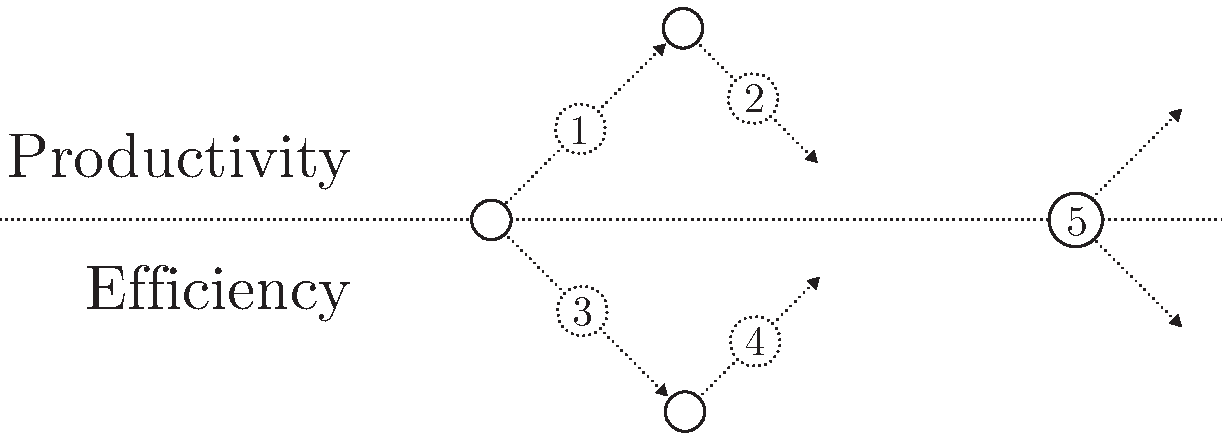
\includegraphics[width=0.6\textwidth]{../ressources/state-of-the-art.pdf}
\end{center}
\end{figure}

\subsection{Web Compliance}

TODO





\section{Productivity Focused Platforms} \label{chapter3:software-productivity}

\cit{It is becoming increasingly important to the data-processing industry to be able to produce
[programming systems] % more programming systems and produce them with fewer errors,
at a faster rate, and in a way that modifications can be accomplished easily and quickly.}{W. Stevens, G. Myers, L. Constantine \cite{Stevens1974}.}

In order to improve and maintain a software system, it is important to holds in mind a mental representation of its implementation \cite{Simon1962}.
As the system grows in size, the mental representation becomes more and more difficult to grasp.
Therefore, it is crucial to decompose the system into smaller subsystem easier to grasp individually.

\cit{Measuring programming progress by lines of code is like measuring aircraft building progress by weight.}{Bill Gates}

Section \ref{chapter3:software-productivity:modularity} presents the modular programming paradigms, and their programming models, oriented toward productivity.
Section \ref{chapter3:software-productivity:adoption} presents the adoption of the implementations of modular programming languages.
Section \ref{chapter3:software-productivity:performance} presents the consequences of the modularity on performance.
Finally, section \ref{chapter3:software-productivity:summary} summarizes the three previous sections in a table.

\subsection{Modular Programming} \label{chapter3:software-productivity:modularity}

\begin{figure}[!h]
\begin{center}
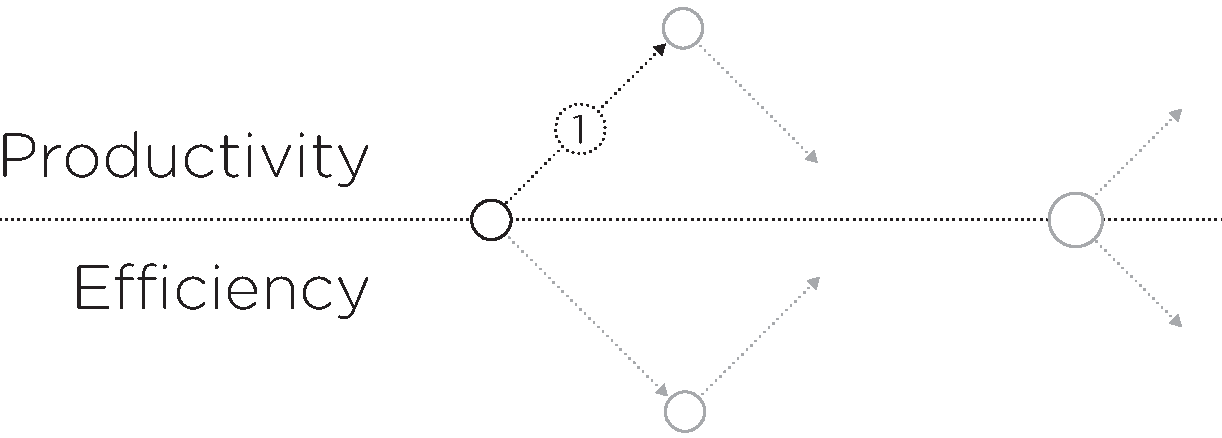
\includegraphics[width=0.6\textwidth]{../resources/state-of-the-art-1.pdf}
\end{center}
\caption{Focus on Productivity}
\label{fig:state-of-the-art-1}
\end{figure}

The next paragraphs presents the different programming model regarding their support to modular programming and productivity.

\subsubsection{Imperative Programming}

\illustration{spaghetti programming}
\illustration{lasagna programming}

Imperative programming is the very first programming paradigm, as it evolves directly from the hardware architectures.
It allows to express the suite of operation to carry sequentially on the computing processor.
Most imperative languages provide encapsulation with modules but not higher-order programming. % , nor lazy evaluation.
The implementations of Imperative Programming are \ImplementationsOf{Imperative Programming}.

\subsubsection{Object Oriented Programming}

\illustration{multiple cells communicating}

The very first Object-Oriented Programming (OOP) language was Smalltalk \cite{Goldberg1984}.
It defined the core concepts as message passing and encapsulation %, and dynamic binding
\ftnt{http://userpage.fu-berlin.de/~ram/pub/pub\_jf47ht81Ht/doc\_kay\_oop\_en}.
Nowadays, the emblematic figures in the software industry are \ImplementationsOf{Object-Oriented Programming}.
They provide encapsulation with Classes, and allows mutable structures for performance reasons.
They recently introduced higher-order programming with lambda expressions.

\subsubsection{Functional Programming} \label{chapter3:software-productivity:programming-models:functional-programming}

% \cit{All problems in computer science can be solved by another level of indirection}{Butler Lampson}

The definition of pure Functional Programming resides in manipulating only expressions and replacing state mutability, with immutable message-passing.
The absence of state mutability makes a function side-effect free, hence their execution can be scheduled in parallel.
The most important pure Functional Programming languages are \ImplementationsOf{Functional Programming}.
They provide encapsulation, higher-order programming and lazy evaluation.

\subsubsection{Multi-Paradigm}

The functional programming concepts are also implemented in other languages along with mutable states and object-oriented concepts.
Major recent programming languages, including Java 8 and C++ 11, now commonly present \textbf{higher-order functions}.
\textit{In fine}, it helps developers to write applications that are more maintainable, and favorable to evolution \cite{Hughes1989,Turner1981}.
These recent multi-paradigms languages such as \ImplementationsOf{Multi Paradigm} combine the different paradigms to help developer building applications faster.

\separator

The previously presented programming models are all rather focused on productivity, as recapped in table \ref{tab:productivity-modularity}.

\ModularProductivityTable{tab:productivity-modularity}

\subsection{Adoption} \label{chapter3:software-productivity:adoption}

As stated previously, adoption relies an productivity as well as efficiency.
The next paragraphs presents the adoptions of different platforms for web development and focus on Javascript.

\begin{figure}[!h]
\begin{center}
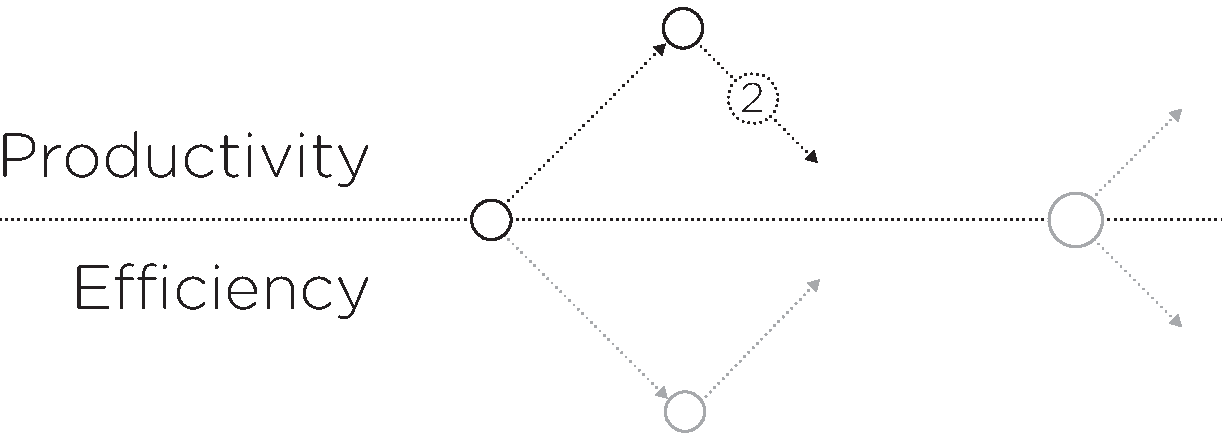
\includegraphics[width=0.6\textwidth]{../resources/state-of-the-art-2.pdf}
\end{center}
\caption{Steering back toward Performance Efficiency}
\label{fig:state-of-the-art-2}
\end{figure}

\subsubsection{Community}

\paragraph{Available Resources}

As of December 2015, Javascript ranks 8th according to the TIOBE Programming Community index, and was the most rising language in 2014.
This index measure the popularity of a programming language with the number of results on many search engines.
And it ranks 7th on the PYPL.
The PYPL index is based on Google trends to measure the number of requests on a programming language.

From these indexes, the major programming languages are Java, C++, C, C\# and Python.
These languages are still widely used by their communities and in the industry.

\begin{figure}[h!]
  \centering
  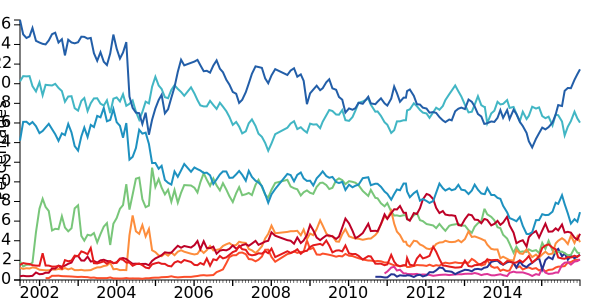
\includegraphics[width=\linewidth]{../resources/tiobe.pdf}
  \label{fig:tiobe}
  \caption{TIOBE ranking}
\end{figure}

\paragraph{Developers Collaboration Platforms}

Online collaboration tools give an indicator of the number of developers and projects using certain languages.
Javascript is the most used language on \textit{Github}\ftnt{the most important collaborative development platform gathering about 9 millions users.} and the most cited language on \textit{StackOverflow}\ftnt{the most important Q\&A platform for developers.}.
It represents more than \num{320000} repositories on \textit{Github}.
The second language is Java with more than \num{220000} repositories.
It is cited in more than \num{960000} questions on \textit{StackOverflow} while the second is Java with around \num{940000} questions.
And according to a survey by \textit{StackOverflow}, it is currently the language the most popular\ftnt{http://stackoverflow.com/research/developer-survey-2015}.
Moreover, the Javascript package manager, \textit{npm}, has the most important and impressive package repository growth.

\begin{figure}[h!]
  \centering
  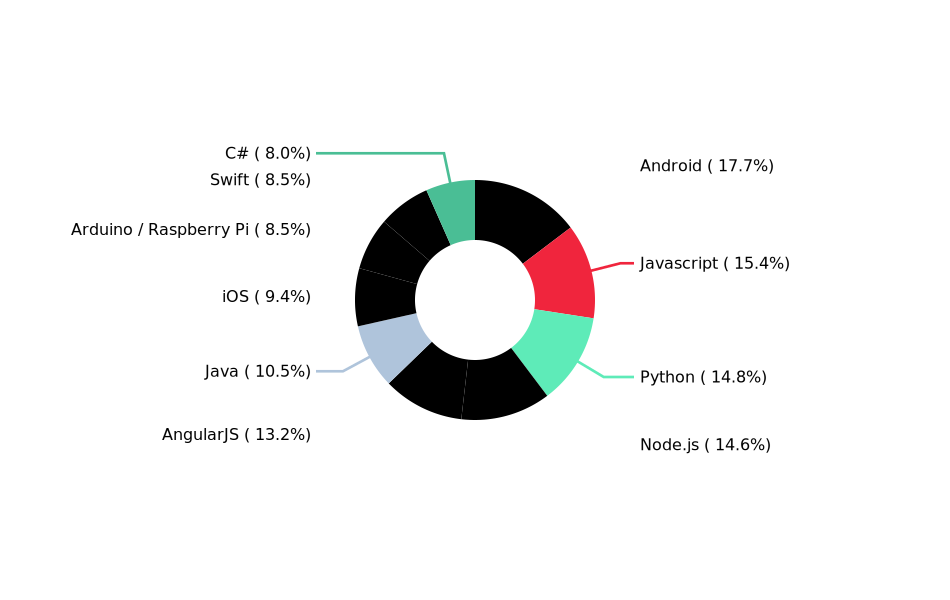
\includegraphics[width=0.7\linewidth]{../resources/stackoverflow-mostwanted.pdf}
  \label{fig:so-tags}
  \caption{Most Wanted Technologies in 2015 from a StackOverflow survey}
\end{figure}

\begin{figure}[h!]
  \centering
  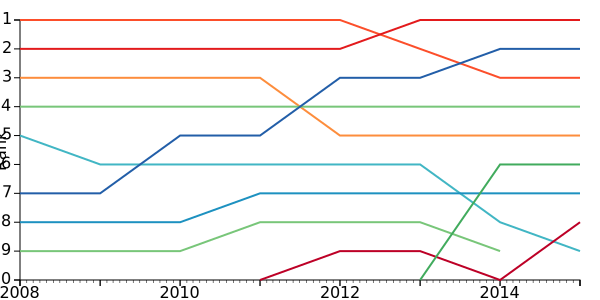
\includegraphics[width=\linewidth]{../resources/github-languages.pdf}
  \label{fig:github-languages}
  \caption{Languages Ranks from number of Github projects}
\end{figure}

\begin{figure}[h!]
  \centering
  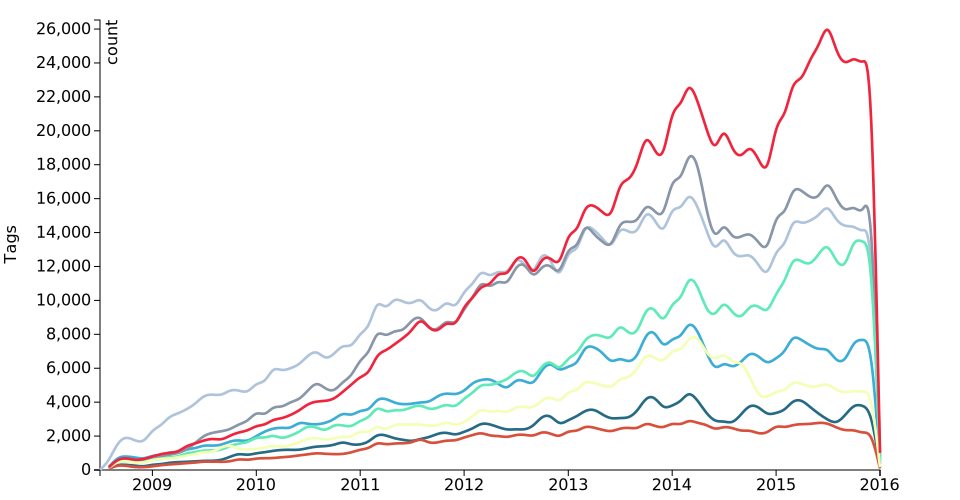
\includegraphics[width=\linewidth]{../resources/stackoverflow-tags.pdf}
  \label{fig:so-tags}
  \caption{StackOverflow Tags evolution}
\end{figure}

\begin{figure}[h!]
  \centering
  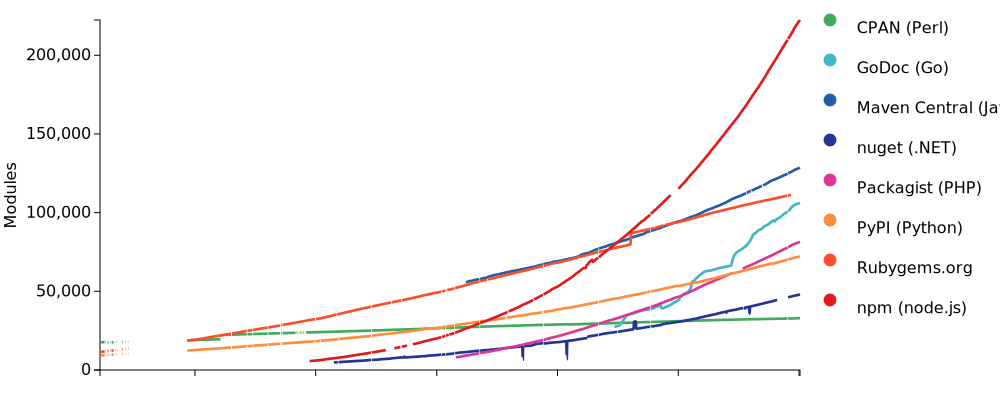
\includegraphics[width=\linewidth]{../resources/modulecounts.pdf}
  \label{fig:modulecounts}
  \caption{Module Counts per package manager}    
\end{figure}

\subsubsection{Industry}

The actors of the software industry tends to hide their activities trying to keep an edge on the competition.
The previous metrics represent the visible activity but are barely representative of the software industry.
The trends on job opportunities give some additional hints on the situation.
Javascript is the third most wanted skill, according to \textit{Indeed}\ftnt{http://www.indeed.com}, right after SQL and Java.\ftnt{http://www.indeed.com/jobtrends?q=Javascript\%2C+SQL\%2C+Java\%2C+C\%2B\%2B\%2C+C\%2FC\%2B\%2B\%2C+C\%23\%2C+Python\%2C+PHP\%2C+Ruby\&l=}
Moreover, according to \textit{breaz.io}\ftnt{https://breaz.io/}, Javascript developers get more opportunities than any other developers.
Javascript is increasingly adopted in the software industry.

\separator

According to these various sources, multi paradigm languages like Javascript are the most widely used by the community and the industry, as presented in table \ref{tab:productivyt-adoption}.
OOP and Imperative Programming remains strong in the industry, but are progressively abandoned by the community.
Functional Programming is not well represented in community nor the industry.

% Table \ref{tab:productivity-adoption} presents a summary of the analysis of the programming models presented in the previous paragraphs.

\ModularAdoptionTable{tab:productivity-adoption}

\subsection{Efficiency Limitations} \label{chapter3:software-productivity:efficiency-limitations}

Eventually, the presented languages are hitting a wall on their way to performance.
They provide global memory abstraction on which to rely to assure encapsulation and composition. % -- either mutable state or immutable state.
Functional programming relies on immutable message-passing.
It might impacts performance at a fine-grain level because of heavy memory usage.
And the synchronization required by mutable state is often hard to develop with \cite{Adya2002}, or avoid parallelism \cite{Pai1999,Krohn2007}.
These results are recapped in table \ref{tab:productivity-performance}.

\ModularEfficiencyTable{tab:productivity-performance}

The only solution to provide performance efficiency is to combine mutable state at a fine-grain level and immutable state at a coarse-grain level \ftnt{http://joeduffyblog.com/2010/07/11/thoughts-on-immutability-and-concurrency/}.
That is to provide both synchronization and message-passing to allow parallelism.
The platforms extending these languages with concurrent or parallel paradigms to improve efficiency are addressed in the next section.

\subsection{Summary} \label{chapter3:software-productivity:summary}

The evaluation of the platforms presented in this section is summarized in table \ref{tab:productivity-synthesis}.

\ModularSummaryTable{tab:productivity-synthesis}















\endinput

Octave and python: higher-level scripting languages productivity and performance evaluation, by Chaves, Nehrbass, Guilfoos, Gardiner.
Haskell vs Ada vs C++ vs Awk vs ... an experiment in software productivity, technical report by Hudak and Jones.
An empirical comparison of seven programming languages, by Prechelt.


remote first Zack Holman : promote asynchronous communication
\ftnt{http://zachholman.com/posts/remote-first/}
+
Conway's law
\cit{Organizations which design systems [...] are constrained to produce designs which are copies of the communication structures of these organizations.}
{M. Conway \cite{Conway1968}}


What makes a great software engineer? \cite{Li2015}

About great software development:
Productivity : Sackman et. al 68, Gugerty & Olson 86
Collaboration, meaningful contribution : Kelly 99, Begel & Simon 06, Hewner & Guzdial 10
Communicate and acquire understanding : LaToza 06, Ko 06
Technical Knowledge : 
Open minded : McConnell 04, Bryant 13


Compiler productivity language into perfomance language
\cite{Kuper2015}\nt{TODO update biblio entry}
\section{Software Efficiency} \label{chapter3:software-efficiency}

\nt{Introduction on the problem of software performance (don't start with the parallelism)}

Programming started with a sequential nature.
The Moore's law \cite{Moore1965} and Dennard's MOSFET scaling \cite{Dennard2007} were wrongly interpreted to promise the exponential evolution in the sequential performance of the processing unit.
 % Programming started with a very sequential nature, as Moore's law \cite{Moore1965} was wrongly interpreted as an exponential evolution in the sequential performance of the processing unit.

% TODO Dennard scaling broke down \cite{Dennard2007}

The first models of computation, like the Turing machine and lambda-calculus, were sequential and based on a global memory state.
A formalism was missing to represent concurrent computations.
This section presents the most important works on formalisms for parallel computation.
They tackled the problems of determinacy, state synchronization and correctness of execution in a formalism based on a network of concurrent processes, asynchronously communicating via messages.
This section first presents the works on the programming models based on this formalism.
Then it presents the huge improvements we recently witnessed in the field of distributed stream processing due to the need of performance from the web to process large stream of requests,

\subsection{Parallel Programming}

\begin{center}
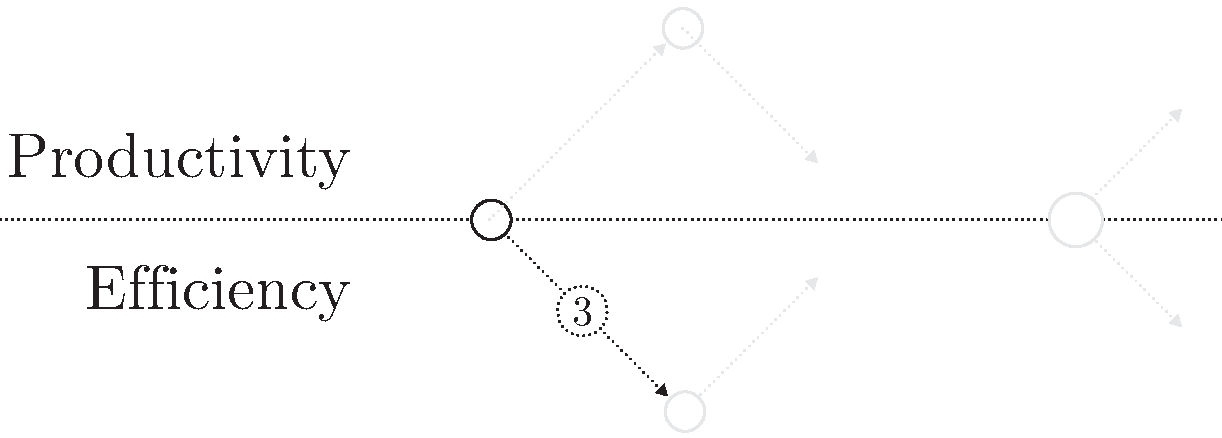
\includegraphics[width=0.6\textwidth]{../ressources/state-of-the-art-3.pdf}
\end{center}

\subsubsection{Execution Causality}

\nt{Causal ordering of execution, instead of global ordering
Causality / Concurrent programming / Asynchronism / Message-passing / Synchronization ...}

Causal ordering of execution, instead of global ordering, lead to concurrent programming, and with some memory synchronization to parallel programming.

% All these early work adopted concurrent composition by default, instead of sequential composition, to adapt to the very concurrent nature of real parallel machines.
% However, sequential programming is still the default.
% Concurrent composition is yet still to be widely accepted, as stated by Reed \cite{Reed2012}.
% \comment{TODO rewrite this paragraph}

% The Actor Model uses asynchronous communications, while $\pi$-calculus uses synchronous communications.
% Synchronous communications are deterministic.
% The message sent needs to be received to continue the execution on both ends.
Because of the synchronous communication used by $\pi$-calculus, the concurrent executions and the communications are both deterministic.
Therefore, the result of the concurrent system is assured to be deterministic.
The correctness of the execution of deterministic systems is guaranteed.
% Determinism is a wanted property to assure the correctness of the execution.

On the other hand, the asynchronous communications used by Actors are non-deterministic.
The message sent can take an infinite time to be received.
Therefore, the result of the concurrent system is not assured to be deterministic.

But the communication in reality are subject to various faults and attacks \cite{Lamport1982}.
And the wait required by synchronous communications negatively impact performances of the system because of the difference of latency between communication, and execution.
The Actor model was explicitly designed to take these physical limitations in account \cite{Hewitt1977a}.
The non-determinism in the asynchronous communications is hidden by the organization of the system.
The total ordering of messages possible with synchronous communication is too strong a requirement for correctness.
As Lamport showed \cite{Lamport1978}, and Reed related later \cite{Reed2012}, causal order is sufficient to build a correct distributed system.
% The non-determinism in the asynchronous communications is hidden by the organization of the system.
The ordering of messages is only local to an actor, while between actors, messages are causally ordered.
The execution will either terminate correctly, or not terminate at all because of a failure in the communications.

Eventually, following works adopted asynchronous communications as it is hardly realistic to build a distributed system based on synchronous communications.




% Asynchronous communications are less expressive than synchronous ones \cite{PALAMIDESSI2003}.

% Pi-calculus is a synchronous paradigm which contains an asynchronous fragment.\cite{PALAMIDESSI2003}
% (Boudol, G. (1992). Asynchrony and the π-calculus (note). Rapport de Recherche  1702, INRIA, Sophia-Antipolis,
% Honda, K. and Tokoro, M. (1991).  An object calculus for asynchronous communication. In America, P., editor, Proceedings of the European Conference on Object-Oriented Programming (ECOOP), volume 512 of Lecture Notes in Computer Science, pages 133–147. Springer-Verlag)


% The asynchronous pi-calculus defined by Honda and Tokoro in 1991 led to Pict, a programming language\cite{Pierce2000}.




% There was firstly theories, and models for concurrent computation.
% The main problem was determinism.
% In a sequential machine, the non-determinism of the physical world is hidden by the sequentiality of the machine.
% However, in concurrent computation, the order of communication cannot be assured the way the order of statements is assured in a sequential machine.
% We observe local non-determinism.
% However, to conserve an apparent determinism, causal ordering is sufficient.




\subsubsection{State Independence}


As demonstrated by the theory, concurrency boils down to causality expressed with message passing.
There exist several programming model over this theoretical view.

\paragraph{Independent Processes}

The theory advocates asynchronous message-passing, but it doesn't precise the granularity of the communicating entities.
In the Actor Model, everything is an actor, even the simplest types, like numbers, similarly in OOP, everything is an object.
In practice, this level of granularity is unachievable due to overhead from the asynchronous communications.
Most implementations adopt a granularity on the process or function level.

% concurrent programming
The first concept using message passing was the coroutine.
% It influenced many following works.
Conway defines coroutines as an autonomous program which communicate with adjacent modules as if they were input and output subroutines \cite{Conway1963}.
It is the first definition of a pipeline to implement multi-pass algorithms.
Similar works include the Communicating Sequential Processes (CSP) \cite{Hoare1978, Brookes1984}, and the Kahn Networks \cite{Kahn1974, Kahn1976}.

% Hoare presented the Communicating Sequential Processes (CSP) \cite{Hoare1978, Brookes1984}.
% These processes are executed concurrently, and communicates events via named channels.
% The evolutions of this model were influenced by, and influenced the work of Milner that led to $\pi$-calculus.

% Similarly, Kahn developed the Kahn Networks \cite{Kahn1974, Kahn1976}, following the work of Conway on coroutines.
% They are explicitly parallel coroutines separated by bounded FIFO streams for communication.

These programming models don't allow to dynamically modify the topology of the application.
Coroutines and processes are defined statically in the source of the application.
We shall come back to this limitation later in this thesis in chapter \ref{chapter5}.

% The shared-nothing architecture \cite{Stonebraker1986}.

As we saw in last section, higher-level programming is helping modularity.
The absence of this feature in the concurrent programming model is a limitation.
On of the instrumental gaol of this thesis is to allow to bring higher-level programming in parallel programming, without the need for manual synchronization, as we will see in the next section.

\paragraph{Synchronization}

\nt{Too raw, not enough synthesis in this section}

These programming models allowed parallel execution on several processing units, so there is a need to shared resources among processing units, like a common memory store, or network interface.
Multiprogramming was used to allow different programs to be executed concurrently in isolated processes, and to share resources \cite{Dijkstra1968}.
To synchronize the different processes over these resources, and avoid conflicting accesses, it is crucial to assure the mutual exclusion.
For this purpose, Djikstra introduced the Semaphore \cite{Dijkstra}.
Similar works include guarded commands \cite{Dijkstra1975}, guarded region \cite{Hansen1978a} and monitors \cite{Hoare1974}.
They are all kinds of locks to assure mutual exclusion.

% Following this work, he also introduced guarded commands \cite{Dijkstra1975} and Hansen introduced guarded region \cite{Hansen1978a}.
% Both assure the execution of a set of instructions to be exclusive to only one process.

% Hoare introduced the monitor following the work of Hansen \cite{Hoare1974}.
% A monitor is an extension of a class, it regroups data and procedures, except that it assures its procedures to be entered only once at a time.
% With this restrictions, it guards against race condition on the access of a shared resource.
% Modula \cite{Wirth1977} and Concurrent Pascal \cite{Hansen1975} uses Monitors.

\subparagraph{Multi-Threading}

As we saw earlier, a common memory storage helps to follow the best practice, and is easier to develop with.
These lock mechanisms were used in Multi-Threading to provide this common memory storage for concurrent programming.
% Multi-threading programming make use of synchronization within isolated processes.
Threads are light processes sharing the same memory execution context within an isolated process.
It seems to be an easy solution to parallelize sequential execution on parallel execution units with a common memory store.
But because of the preemptive scheduling, threads require to lock each and every shared memory cell.
It is known that this heavy need for synchronization leads to bad performances, and is difficult to develop with \cite{Adya2002}.

\subparagraph{Lock-Free Data-Structures}

An interesting alternative to locks are the wait-free and lock-free data-structures \cite{Lamport1977,Herlihy1988,Herlihy1990,Herlihy1991,Anderson1990}.
They are based on clever use of atomic read and write operations on a shared memory to provide concurrent safe version of common data-structures algorithms.
Therefore no locking is necessary for the algorithm to be highly concurrent, while conserving a common memory store
However, even if they are theoretically infinitely scalable, they are hard to come with, and are not fit for every problem.
% Lock-free algorithm are highly concurrent, as they can be replicated, however, they are limited, and really hard to develop.
% \url{https://en.wikipedia.org/wiki/Non-blocking_algorithm}

% Reference papers :
% Concurrent reading and writing \cite{Lamport1977}
% Impossibility and universality results for wait-free synchronization \cite{Herlihy1988}
% A methodology for implementing highly concurrent data structures \cite{Herlihy1990}
% Wait-free synchronization \cite{Herlihy1991}

% Book :
% The virtue of Patience: Concurrent Programming With And Without Waiting \cite{Anderson1990}

\subparagraph{Scalability Limitation}

Amdahl \cite{Amdahl1967} and later Ghunter \cite{Gunther1993} theorized the speedup gains with parallelism for a sequential program.
They concludes that sharing resources protected by mutual exclusion eventually decreases performances when increasing parallelism \cite{Gustafson1988,Gunther1996,Nelson1996,Gunther2002}.

The concurrent process sharing resources need to be scheduled sequentially, and not in parallel, as the contention of locking negatively impact the performance.
To increase the parallelism and performance, it implies to reduce the shared resources between concurrent processes.

% The execution regions requiring the same resource needs to execute sequentially.
% This wait impacts performances negatively because of contention.
% Therefore, to increase parallelism one needs to increase the number of independent processes, and to ensure their communicate to be solely by asynchronous messages without waiting.

\subparagraph{PGAS}

Sharing resources eventually limits scalability, hence distribution of the memory is unavoidable.
The Partitioned Global Address Space (PGAS) model replaces the need for a common memory store.
It provides the developers with a uniform memory access on a distributed architecture.
Each computing node executes the same program, and provide its local memory to be shared with all the other nodes.
The PGAS programming model assure the remote accesses and synchronization of memory across nodes, and enforces locality of reference, to reduce the communication overhead.
% This model is a SPMD : Single Program Multiple Data.
Known implementation of the PGAS model are 
Chapel\cite{Chamberlain2007},
X10 \cite{Charles2005}.
Unified Parallel C \cite{El-Ghazawi2006},
CoArray Fortran \cite{Numrich1998} and
OpenSHMEM \cite{Chapman2010}.

These programming models are promising.
However, they focus rather on scientific application with intensive computing such as matrix multiplication, and leave out streaming applications, such as web services.

\paragraph{Programming languages} \label{chpater3:concurrent-programming:programming-languages}

% Scala / Akka / Erlang

Some programming languages features message-passing and isolation of actors directly to give the responsibility to developers to assure high parallelism.
To some extent, these languages succeeded in industrial contexts.
However, they largely remain elitist solutions for specific problems more than a general, and accessible tool.
I present some examples below.

Scala is an attempt at unifying the object model and functional programming \cite{Odersky2004}.
% It proposes an actor approach in its design.
Akka\ftnt{http://akka.io/} is a framework based on Scala, to build higly scalable and resilient applications.

Erlang is a functional concurrent language designed by Ericsson to operate telecommunication devices \cite{JoeArmstrong,Nelson2004} % Nelson2004 is not very good, find another better citation.

CUDA, OpenCL are data parallel API to allow imperative code to run onto accelerators such as GPUs or FPGAs \cite{Stone2010}.

The field of concurrent programming is so vast it is impossible to relate here every of its branch.
The previous examples are only the best known.
The next focus focuses on streaming real-time applications.






\paragraph{Stream Processing Systems} \label{chapter3:parallel-execution:stream-processing}

All the solutions previously presented are designed to build general distributed systems.
We focus on real-time applications as defined by \cite{Hansen1978}.
A real-time application must respond to a variety of simultaneous requests within a certain time.
Otherwise, input data may be lost or output data may lose their significance.
Such applications are often connected to the internet and use the web as an interface, which implies to process high volumes streams of requests.
Moreover, because these systems are key to business, their reliability and latency are of critical importance.
These requirements are challenging to meet in the design of such system.
It present the state of the art to design such systems with these challenging requirements.


% \textit{
% From a language designer's point of view, real-time
% programs have these characteristics:
% \begin{enumerate}
% \item A real-time program interacts with an environ-
% ment in which many things happen simultaneously at
% high speeds.
% \item A real-time program must respond to a variety
% of nondeterministic requests from its environment. The
% program cannot predict the order in which these requests
% will be made but must respond to them within certain
% time limits. Otherwise, input data may be lost or output
% data may lose their significance.
% \item A real-time program controls a computer with a
% fixed configuration of processors and peripherals and
% performs (in most cases) a fLxed number of concurrent
% tasks in its environment.
% \item A real-time program never terminates but contin-
% ues to serve its environment as long as the computer
% works. (The occasional need to stop a real-time program,
% say at the end of an experiment, can be handled by ad
% hoc mechanisms, such as turning the machine off or
% loading another program into it.)
% \end{enumerate}
% }

\subparagraph{Data-stream management systems}

% The processing of large volume of data was historically handled by Database management systems.
% These systems naturally evolved to manage data-streams as well.

Database Management Systems (DBMS) historically processed large volume of data, and they naturally evolved into Data-stream Management System (DSMS) to processed data streams as well.
They concurrently run SQL-like requests on continuous data streams.
The computation of these requests spread over a distributed architecture.
Among the early works, we can cite NiagaraCQ \cite{Chen2000,Naughton2001}, Aurora \cite{Abadi2003,Abadi2003a,Balakrishnan2004} which evolved into Borealis \cite{Abadi2005}, AQuery \cite{Lerner2003}, STREAM \cite{Arasu2003,Arasu2005} and TelegraphCQ \cite{Krishnamurthy2003,Chandrasekaran2003}.
More recently, we can cite DryadLINQ \cite{Isard2007,Yu2009}, Timestream \cite{Qian2013} and Shark \cite{Xin2013}.

However, these solutions implies to understand two paradigms of language, the SQL paradigm, and the imperative paradigm.
% Even if SQL is a turing-complete language, it is rather difficult to write a complex application only with a SQL-like language.
The difference between these two paradigms creates a rupture in the design of the system.
% Even if the design follows an imperative structure,
The SQL parts difficulty merge with the imperative structure.
% It is harder to separate concerns. \nt{need reference, plus rewrite this paragraph}.
This rupture impacts the maintainability of the system as it is not straightforward to reorganize the logic between the two paradigms.


% SQL-like
%   AQuery \cite{Lerner2003}
%   STREAM (uses CQL) \cite{Arasu2003,Arasu2005}
%   TelegraphCQ (uses StreaQuel) \cite{Krishnamurthy2003,Chandrasekaran2003}
%   Grape / Timestream - distributed SQL (roughly) \cite{Qian2013}
%   Shark        Stateless dataflow \cite{Xin2013}

%   DryadLINQ    Stateless dataflow \cite{Isard2007,Yu2009}

% \subsubsection{Batched dataflow}

% Map/Reduce
%   MapReduce    Stateless dataflow \cite{Dean2008}
%   Hadoop       Stateless dataflow 
%   Incoop       Incremental dataflow \cite{Bhatotia2011}

% Functional
%   Comet        Batched dataflow \cite{He2010}
%   D-Streams    Batched dataflow \cite{Zaharia2012}
%   Spark        Stateless dataflow \cite{Zaharia,Zaharia2010}
%   Nectar       Incremental dataflow \cite{Gunda2010}



\subparagraph{Dataflow pipeline} \label{chapter3:software-efficiency:dataflow-pipeline}

An alternative model to process data stream efficiently is the pipeline architecture.
It inspires from dataflow to integrate the two conflicting programming paradigms into one.

SEDA is a precursor in the design of pipeline-based architecture for real-time applications for the internet \cite{Welsh2001}.
It organizes an application as a network of event-driven stages connected by explicit queues.
It is based on previous works \cite{Gribble2001,Pai1999}.

Several projects followed and adapted the principles in this work.
StreaMIT is a language to help the programming of large streaming application \cite{Thies2002}.
Storm \cite{Toshniwal2014} is designed by and used at Twitter calculate metrics on streams of tweets such as the trending topics.
% It is only one example of industrial practical application, among many others.
Among other works, there are CBP \cite{Logothetis2010} and S4 \cite{Neumeyer2010}, that were designed at Yahoo, Millwheel \cite{Akidau2013} designed at Google and Naiad \cite{Murray2013} designed at Microsoft.

Similarly to the programming models presented in section \ref{chpater3:concurrent-programming:programming-languages} these frameworks are elitist and not accessible to a large community of developers.
Indeed, the pipeline architecture present a distributed storage, which is hardly compatible with the best practices.
It impacts maintainability.
For this reason, there are some works on reconciling the concurrent programming models with the modular programming model favoring maintainability.
The next section presents these reconciliations.

% Dataflow
%   CBP          Incremental dataflow \cite{Logothetis2010}
%   S4           Continuous dataflow \cite{Neumeyer2010}
%   Storm        Continuous dataflow \cite{Toshniwal2014}
%   Millwheel    Continuous dataflow \cite{Akidau2013}
%   SEEP         Continuous dataflow \cite{Fernandez2013}
%   Naiad        Batched dataflow \cite{Murray2013}



Transition on the limitations of software parallelism)

\subsection{Maintainability Improvements}

\begin{center}
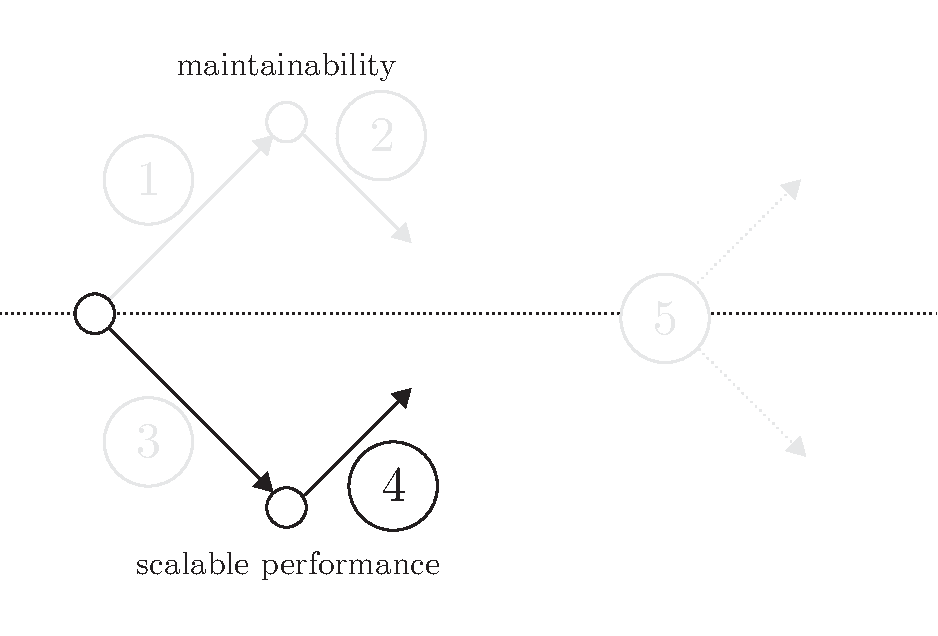
\includegraphics[width=0.6\textwidth]{../ressources/state-of-the-art-4.pdf}
\end{center}

\subsubsection{Design Patterns}

Algorithm skeleton (Map/Reduce ... )

As we explained in the previous sections, the two different organization, modular and parallel, seems intuitively incompatible.
However, it might be possible to find specific organizations that are both modular and parallel, and fit both requirements of maintainability and performance.
% fit both concerns for particular cases.

Algorithmic skeletons are general computational framework for distributed computing proposing predefined patterns that fit certain type of problems \cite{Cole1988, Dean2008, McCool2010, Gonzalez-Velez2010}.
A developer expresses its problem as a specific case of a skeleton.
It simplifies the design and implementation of the communications, hence the developer can focus on its problem independently of the distributed communications, and their performance overhead.

As there is similtudes between SQL-like languages, functional structures, and algorithmic skeletons, the latter can be seen as a tentative to merge the more descriptional features of the former into imperative programming.
Indeed, among the Algorithmic skeletons, we can cite Map / reduce, which are functional structures, but are somehow equivalent to the select and aggregate functions of SQL.
The pipeline architecture for data stream processing presented in section \ref{chapter3:software-efficiency:dataflow-pipeline} can be considered as algorithmic skeletons.

However, they introduce limitations and difficulties, as the developer must fit its problem into the skeletons.
% One of this difficulties, it that a common memory is impossible to use.
Developers needs to think in terms of message passing instead of a global memory, which, as we saw in previous section, is incompatible with best practices.

\subsubsection{Granularity}

Microservices, SOA ...


Another approach in an industrial context is the Service Oriented Architectures (SOA).
It allows developers to express an application as an assembly of services connected to each others.
It shows well the difference between Information Hiding Principles and Separation of Concerns, as a service doesn't encapsulate a design choice, but a specific task.
SOA is in contradiction with the former, but consistent with the latter.

More recently, in the web service development communities, emerged the term of microservices, following the trends of SOA.
It to choose and deacrease the granularity of the fitting between modular organization and parallel execution.
Using Microservices implies that software developers can manage the two organizations at a sufficiently fine level.
As said in section \ref{chpater3:concurrent-programming:programming-languages} and \ref{chapter3:software-efficiency:dataflow-pipeline}, it is an elitist point of view.
Most developers are unable to manage efficiently the two organizations.

Moreover, in these solutions, higher-order programming is impossible.
As we showed earlier in section \ref{chapter3:software-design:programming-models:functional-programming}, higher-order programming is important for modular design and maintainability.
The next section present some work on compiling from one organization into the other.
By keeping the modular programming model, the compilation approach allows higher-level programming. 

\nt{TODO EJB}

\subsubsection{Lack of Higher-Order Programming}

\paragraph{Transistion : these methods doesn't allow higher-order programming, which is required for good modularity.}


\endinput

\subsection{Concurrency Theory} \label{chapter3:parallel-execution:concurrency-theory}

The mathematical models are a ground for all following work on concurrent programming, we briefly explain them in the next paragraphs.
There are two main formal models for concurrent computations.
The Actor Model of C. Hewitt and the Pi-calculus of R. Milner.
Based on these definitions, we explain the importance of determinism for correctness, and the reasons that made asynchronous message-passing prevail.

% TODO illustration of cells, and draw an analogy between cells and actor model.
% Or something the actor models is based upon.

\subsubsection{Models}

\paragraph{Actor Model}

The Actor model allows to express the computation as a set of communicating actors \cite{Hewitt1973a, Hewitt1977, Clinger1981}.
In reaction to a received message, an actor can create other actors, send messages, and choose how to respond to the next message.
All actors are executed concurrently, and communicate asynchronously.
% The Actor model uses an asynchronous message-passing communication paradigm.
% The communication between two actors, the sender and the receiver, is a stream of discrete messages.
% The sender names the receiver actor when sending messages to be the recipient of these messages.
An asynchronous communication implies that the sender continues its execution immediately after sending the message, before receiving the result of the initiated communication.

The Actor model was presented as a highly parallel programming model, but intended for Artificial Intelligence purposes.
Its success spread way out of this scope, and it became a general reference and influence.
% For example, the Scala programming language features an actor approach to concurrency.

% More recent work of C. Hewitt on Actors is about ... \nt{TODO} \cite{Hewitt2007,Hewitt2007a}.

\paragraph{$\pi$-calculus}

R. Milner presented a process calculus to describe concurrent computation : the Calculus of Communicating Systems (CCS) \cite{Milner1975, Milner1980}.
It is an algebraic notation to express identified processes communicating through synchronous labeled channels.
% In CCS, process compose concurrently, communications are synchronous, and the topology is static.
The $\pi$-calculus improved upon this earlier work to allow processes to be communicated as values, hence to become mobile \cite{Engberg1986,Milner1992a,Milner1992}.
Therefore, similarly to Actors, in Pi-calculus processes can dynamically modify the topology.
However, contrary to the Actor model, communications in Pi-calculus are based on simultaneous execution of complementary actions, they are synchronous.


% Actors can create actors, pi-caclulys processes can replicate, and send processes through channel.
% Processes create a new processes on each instruction to continue the execution.!g systolic arrays

% Pi-calculus resembles to the actor model, but its algebraic nature led to a critical difference with the latter.
% Indeed, processes in the Pi-calculus communicate indirectly, through labeled ports, whereas actors communicate directly by naming the recipient actors.
% This difference allows multiple processes to listen in turns to the same channel, whereas the recipient of a message cannot change.

% I think this difference lead the Pi-calculus to be composable, whereas message-passing is not.
% Message-passing is not composable, whereas invocation is.
% The Actor model is not an ideal programming model, as non-composability makes difficult to reuse or extends existing components.
% A way to compose actors, is to send to an actor the name of the actor to respond to.
% It is similar in essence to the continuation concept.








\section{Reconciliations} \label{chapter3:reconciliations}
\nt{TODO title not clear enough}

\subsection{Contradiction}

The decomposition of an application into a pipeline, as shown in the two previous sections, is incompatible with the modular design advocated by the separation of concerns.
The problem of incompatibility between the modular design and the parallel execution of a pipeline architecture is the following.
There need to be a common understanding on the structure of the communication from one stage to the next.
The modular design defines that this common ground, the interface, be the most resilient possible to focus the evolution within a module.
While the pipeline architecture (and more generally the concurrent programming models) defines these interfaces as the communications between the stages of the execution.
With the evolution of the problem specification, when a stage needs to be modified, it is most likely that these changes will affect the previous or next stages.
% which will eventually change with the evolution of the problem specification.

Most project use languages supporting the modular design at the beginning, when they need to evolve the most.
They then switch to the pipeline architecture only when the requirement of performance overcomes the requirement of evolution.
Moreover, as the team knows that they will eventually throw away their code to upgrade it to a different paradigm, there is little effort to follow the best practice to make maintainable code.
It results in a large effort of development to compensate this rupture.
% This rupture between the two organization is not novel, and is at the center of a large body of work.
In this section, we present the state of the art to reconciliate the two organizations, and avoid this rupture.
First we see the design patterns to fit both organization onto a same source code.
Then we see the compilation tentatives to switch from one to the other.










TO READ :

Streaming
\cite{Madsen2015}
\cite{Sun2015}

Map Reduce
\cite{Yao2015}


Web assembly
https://medium.com/javascript-scene/what-is-webassembly-the-dawn-of-a-new-era-61256ec5a8f6
\section{Adoption Focused Platforms} \label{chapter3:software-adoption}

The platforms previously presented focus on productivity or efficiency.
The previous section concludes that favoring one negatively impacts the other.
Moreover, a balance between productivity and efficiency is required to be both supported by the community and needed by the industry, hence trigger a virtuous circle of adoption.
Some platforms feature an abstraction of the task organization to allow developers to focus on the modular organization to keep both productivity and efficiency.
This abstraction happens either at compile time or at runtime.

% \nt{read and include \cite{Catanzaro2009} it is about Productivity language JIT compilation into efficient language
% And get all the paper that cite this one.}
% \nt{read and include \cite{Engler1994}}
% \nt{read and include \cite{Kovachev2011}}
% \nt{read and include \cite{Asanovic2006}}

\begin{figure}[h!]
\textfig{%
  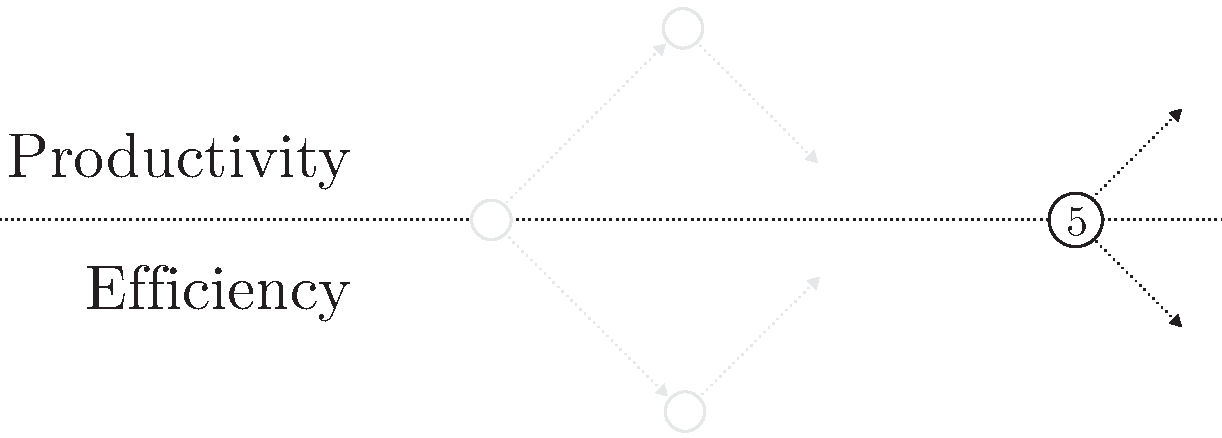
\includegraphics[width=0.6\textwidth]{../resources/state-of-the-art-5.pdf}%
  \caption{Focus on Adoption}%
  \label{fig:state-of-the-art-5}%
}%
\end{figure}

\subsection{Abstraction of Tasks Organization}

\subsubsection{Compilers} \label{chapter3:software-adoption:compilers}

\cit{It is a mistake to attempt high concurrency without help from the compiler.}{R. Behren, J. Condit, E. Brewer \cite{Behren2003}}

The idea to bridge the gap between the tasks and modules organizations dates from the initial paper that presented this gap \cite{Parnas1972}.
However, the implementation of this idea remains a work in progress.

% read and include \cite{Catanzaro2009}

\paragraph{Parallelism Extraction}

To extract parallelism from a sequential implementation, a compiler needs to identify the commutative operations to parallelize their executions \cite{Rinard1996,Clements2013a}.
The parallelization of loop iterations has been thoroughly studied \cite{Mauras1989,Amarasinghe1995,Chen2008,Banerjee2013,Radoi2014}, particularly with the polyhedral compilation method \cite{Bastoul2004}.
Examples of polyhedral compilers are \ImplementationsOf{Polyhedral Compilers}.
To improve performance gains outside of loops, some compilers identify parallelism in the data-flow representation on the whole program \cite{Beck1991,Catanzaro2009,Li2012}.

Data processing applications \cite{Fernandez2014a} such as web services \cite{Salmito2013} are often already organized as data-flow.
In higher-order programming, continuous passing style and promises encourage this data-flow organization.
However, the mutable closures required for higher-order programming remains a challenge to parallelize because they rely on a globally shared memory \cite{Harrison1989, Nicolay2010, Matsakis2012a}.
To extract parallelism, compilers rely on static analysis or notations from the developers.

% TODO Extract parallelism compilers from these :
% Load balanced pipeline parallelism \cite{Kamruzzaman2013},
% Regent \cite{Slaughter2015},
% Cilk-P, On-the-Fly Pipeline Parallelism\cite{Lee2013}
% Commutativity analysis: A new analysis framework for parallelizing compilers \cite{Rinard1996}
% Introducing 'Bones': a parallelizing source-to-source compiler based on algorithmic skeletons \cite{Nugteren2012}
% \cite{Herrmann2000}

\paragraph{Static analysis}

Compilers analyze the source code of a program to detect commutative operations in the control flow \cite{Allen1970}.
The point-to analysis is a static analysis method.
It identifies multiple symbolic names pointing to the same memory location.
That is called aliasing.
Hence it idenfities side-effects \cite{Andersen1994,Jang2009,Sridharan2012,Wei2014} between operations, which allows to infer their commutativity.
Another method, the abstract interpretation, is to interpret the possible path of executions with virtual inputs.
It allows to statically reason on the behavior of dynamic programs \cite{Maffeis2008,Smith2011,Gardner2012,Hackett2012,Raychev2013,Gardner2013,Bodin2014}.
It is successfully used for security applications to detect malicious scripts, or obfuscate code \cite{Huang2004,Jovanovic2006,Yu2007,Maffeis2009a,Chudnov2015,Dolby2015}
% \nt{Update the citation for Dolby2015}.

However, these static analysis methods remains often too imprecise, and expensive for the performance gain to be profitable in dynamic languages, such as Javascript \cite{Shivers1991}.
Instead, some compilers relies on annotations from the developers.

\paragraph{Annotations}

Some works proposed to rely on annotations from the developer to identify the shared data structures and infer the commutativity of operations \cite{Vandierendonck2010a,Fernandez2014a}.
Such annotations are especially relevant for accelerators such as GPUs or FPGAs, because the development effort yields huge performance improvements \cite{Tarditi2006}.
Examples of such compilers are \ImplementationsOf{Annotation Compilers}.

% Bloom declarative language \ftnt{http://bloom-lang.net/}
% Blazes: Coordination analysis for distributed programs \cite{Alvaro2014}

\paragraph{Compilation Limitations}

For dynamic languages like Javascript, the static analysis is not sufficient to correctly infer the independence of tasks to parallelize them.
Parallel compilers often fall back on relying on annotations provided by developers.
Hence, the burden of detailing the tasks and memory organizations falls back to the developer.
It impacts productivity and adoption.

\subsubsection{Runtimes} \label{chapter3:software-adoption:runtimes}

At runtime, the incertitudes on the independence of tasks is resolved.
It allows analyzes precise enough to detect and distribute the commutative operations.

\paragraph{Partitioned Global Address Space}

The Partitioned Global Address Space (PGAS) provides a uniform access on a distributed memory architecture.
It attempts to combine the efficiency of distributed memory systems, with the productivity of shared memory systems.
Each computing node executes the same program, and provides its local memory to be shared with all the other nodes.
The PGAS platform assures the remote accesses and synchronization of memory across nodes.
Examples of implementations of the PGAS model are \ImplementationsOf{Partitioned Global Address Space}.

\paragraph{Dynamic Distribution of Execution}

Following SEDA, Leda proposes a model where the independent stages of the pipeline are defined only by their role in the application \cite{Salmito2013,Salmito2014}.
The execution distribution and module organization are different.
The actual execution distribution is defined automatically during deployment.
This automation manages the execution organizations to help the developer focus on the modular organization.
% However, it doesn't improve the composition of module with higher-order programming.

\subsubsection{Productivity and Efficiency}

The platforms presented in this section intend to merge both productivity and efficiency in a single platform by bringing parallelism to productivity languages.
Because they are based on productivity languages, they feature decent encapsulation, but they limit the use of higher-order programming between tasks to allow their isolation.
Hence, it degrades composition, as presented in table \ref{tab:adoption-productivity}.

Despite worse productivity, this parallelization bring good efficiency, as presented in table \ref{tab:adoption-efficiency}.

\AbstractionProductivityTable{tab:adoption-productivity}
\AbstractionEfficiencyTable{tab:adoption-efficiency}

\subsection{Limitation}

The platforms presented in this section come from the need of the industry to reduce the development commitment required for efficiency.
However, these platforms respond exclusively to academic or industrial needs, and are barely supported by the community, as presented in table \ref{tab:adoption-efficiency}.

The balance between efficiency and productivity is not sufficient for a community of passionate to arise.
To be largely adopted, the platforms need to allow novice to start learning and experimenting at small scale.
It incites the community to start projects, and grow them organically to build businesses.
The context of web development is particularly adapted for this growth.

\AbstractionAdoptionTable{tab:adoption-efficiency}

\subsection{Summary}

As detaild in table \ref{tab:adoption-summary}, this section proved that a platform cannot trade productivity against efficiency without massively losing the community required to trigger the adoption.

\AbstractionSummaryTable{tab:adoption-summary}











\endinput



\section{Analysis}

This chapter presented a broad view of platforms and their balance between productivity or efficiency.
The platforms favoring one sacrifice the other.
The adoption, and usage of these platforms prove that none of these compromises are sustainable.

The productive platforms are highly adopted.
Their productivity feed a reinforcing circle of adoption between the community and the industry.
However, they lack the efficiency required to strive in the latter stage of a project, where efficiency becomes crucial.

On the other hand, the efficient platforms are not widely adopted by the community.
These platforms are unable to respond to the need of the community to prototype and to experiment on small projects to make them evolve into larger ones later on.


\paragraph{Continuous Development}

It is not possible for a platform to support both productivity and efficiency at the same time.
These platforms are oriented toward productivity, efficiency or a compromise between both.
As the two are required at different time in the evolution of the project, to follow a project, a platform need to meet the requirements at the good time.
They need to supporting productivity to allow the community to experiment, and organically start projects.
And then continuously shift toward efficiency as the project evolve, and requires it.

None of these platforms are able to support productivity then efficiency to follow the evolution of a project.
They lack the possibility to make a project evolve from the very early stage until maturation. 
A project needs to change platform to change the priority.
These shifts of platforms have economical consequences.

\paragraph{}

The table \ref{tab:summary} summarizes the analysis of the state of the art presented in this chapter.

\TableSummary{tab:summary}

%-----------------------------------------------------------------------------%
                                    \endinput
%-----------------------------------------------------------------------------%


Some links I NEED to put :
--------------------------

https://glyph.twistedmatrix.com/2014/02/unyielding.html
http://calculist.org/blog/2011/12/14/why-coroutines-wont-work-on-the-web/

Transitions :
  - Linkedin - http://engineering.linkedin.com/architecture/brief-history-scaling-linkedin
  - Facebook - https://www.cs.princeton.edu/events/event/evolution-software-architecture-facebook / http://www.infoq.com/presentations/Evolution-of-Code-Design-at-Facebook
  - ... 

https://medium.com/@benorama/the-evolution-of-software-architecture-bd6ea674c477

https://en.wikipedia.org/wiki/Dataflow
https://en.wikipedia.org/wiki/Real-time_computing
https://en.wikipedia.org/wiki/Partitioned_global_address_space
https://en.wikipedia.org/wiki/SPMD

Albert Cohen
https://scholar.google.com/citations?user=MkKZKAMAAAAJ&hl=en

+ Paul Feautrier (Tutor of A. Cohen)


Similar problem :
http://2015.splashcon.org/event/splash2015-splash-i-lindsey-kuper-talk
http://www.cs.indiana.edu/~lkuper/papers/lindsey-kuper-dissertation.pdf

PJS was abandoned :
https://groups.google.com/forum/#!topic/mozilla.dev.tech.js-engine/H-YEsejE6DA
https://bugzilla.mozilla.org/show_bug.cgi?id=1117724

See parallel JS for further work (maybe) :
http://smallcultfollowing.com/babysteps/blog/2014/04/24/parallel-pipelines-for-js/

Some chunks I might find useful later :
---------------------------------------

A good example of declarative sentence in everyday world : in case of fire, 
the elevators don't work -> you understand that you need to take the stairs.